\chapter[Title of the chapter 6 displayed \\ in the table of contents]
    {Title of the chapter 6 displayed in the page
        \chaptermark{Ch. 6 title in the header}
    }
    \chaptermark{Ch. 6 title in the header}
\label{ch:labelchapter6}

\updatemylof % to be used with "list of figure divider per chapter" (see PREAMBLE)
\updatemylot % to be used with "list of table divider per chapter" (see PREAMBLE)

\regularsection
\headerregularsection

Author 1\textsuperscript{1,\textcolor{sophia}{$\ast$}}, Author 2\textsuperscript{1,2,\textcolor{sophia}{$\ast$}}, Author 3\textsuperscript{3}, Author 4\textsuperscript{1}, Author 5\textsuperscript{1}, Author 6\textsuperscript{1}, Author 7\textsuperscript{2,4,\#} and Author 8\textsuperscript{1,\#} \hfill  \newline

\let\thefootnote\relax\footnotetext{\textsuperscript{1}Department X, University 1, City A, Country B. 
\textsuperscript{2}Department Y, University 2, City C, Country D. 
\textsuperscript{3}Institute E, City F, Country G. 
\textsuperscript{4}Research Center H, University I, City J, Country K. 
\textsuperscript{\#}e-mail: \href{mailto:author7@university2.ac.countryD}{author7@university2.ac.countryD} and \href{mailto:author8@universityI.countryK}{author8@universityI.countryK}}

\noindent First published in: \textit{Scientific Reports} \textbf{10}, 853 (2020). \hfill \break
DOI: \href{https://doi.org/10.1038/s41598-019-55424-z}{10.1038/s41598-019-55424-z} 

\begin{wrapfigure}[3]{l}{0.2\textwidth}
    
\includegraphics[width=0.2\textwidth]{figures/by.png}
\end{wrapfigure} 

\noindent \textcolor{white}{test} \newline \textbf{Open Access} This article is licensed under a Creative Commons Attribution 4.0 International License. It means that unrestricted use, sharing, adaptation, distribution, and reproduction in any medium or format are allowed, as long as the original author(s) and the source are appropriately credited, a link to the Creative Commons license is provided, and any changes made are indicated. To view a copy of this license, please visit \href{http://creativecommons.org/licenses/by/4.0/}{http://creativecommons.org/licenses/by/4.0/}. \newline

\noindent \copyright \ Liudi Mulyo \textit{et al}, 2020. \newline

\noindent \textbf{Contributions} \newline
\noindent \lipsum[2]

%%%%%%%%%%%%%%%%%%%%%%%%%%%%%%%%%%%%%%%%%%%%%%%%%%%%%%%%%%%%%%%%%%%%%%%%%%%%%%%%%%%%%%%%%%%%%%%%%%%%%%%%%%%%%%%%%%%%%%%%%%%

\tcbset{enhanced,colback=abstractback,colframe=sophia,fonttitle=\bfseries}
\begin{tcolorbox}[left=3.35cm,grow to left by=3.5cm,right=3.33cm,grow to right by=3.5cm,title={\normalfont \color{White} \small \fontfamily{bch} \selectfont \scshape Abstract}]
% https://tex.stackexchange.com/questions/232878/inserting-pictures-in-tcolorbox
% https://tex.stackexchange.com/questions/169794/outer-margin-of-tcolorbox/169877
% https://tex.stackexchange.com/questions/11484/how-to-draw-a-frame-box-around-an-arbitrary-large-piece-of-text-figures-whatever
\begin{minipage}[t]{\linewidth}
\vspace*{-29pt}
\phantomsection % to fix wrong hyperref to "Abstract" 
\section*{} % for linking from TOC (only one way)
\addcontentsline{toc}{section}{Abstract}
\begin{sloppypar}
\lipsum[1]
\end{sloppypar}

\end{minipage}

\vspace*{3.5pt}
\end{tcolorbox}

%%%%%%%%%%%%%%%%%%%%%%%%%%%%%%%%%%%%%%%%%%%%%%%%%%%%%%%%%%%%%%%%%%%%%%%%%%%%%%%%%%%%%%%%%%%%%%%%%%%%%%%%%%%%%%%%%%%%%%%%%%%

\begin{sloppypar} % to suppress overfull box

As in \Autoref{ch:labelchapter5}. Lorem \index{Lorem} ipsum dolor sit amet, consectetuer adipiscing elit \cite{LIUDIMULYO201767}. Ut purus \index{purus} elit,vestibulum ut, placerat ac, adipiscing vitae, felis \citenum{LIUDIMULYO201767}. Curabitur dictum \index{dictum} gravidamauris. Nam arcu libero, nonummy eget, consectetuer id, vulputate a, magna. Donec vehicula augue eu neque \cite{liudimulyo_2018}. Pellentesque habitant morbi tristique senectuset netus et malesuada fames ac turpis egestas \index{egestas}\citenum{liudimulyo_2018}. Mauris ut leo. Cras viverra metusrhoncus sem \cite{2019liudimulyo}. Nulla et lectus vestibulum urna fringilla ultrices. Phasellus eutellus sit amet tortor gravida placerat \citenum{2019liudimulyo}. Integer sapien est, iaculis in, pretium quis,viverra ac, nunc. Praesent eget sem vel leo ultrices bibendum \cite{liudimulyo2020853}. Aenean faucibus. Morbi dolor nulla, malesuada eu, pulvinar at (\ref{fig:figures/paper-iv/fig-6}), mollis ac, nulla. Curabitur auctorsemper nulla \citenum{liudimulyo2020853}. Donec varius orci eget risus. Duis nibh mi, congue eu, accumsaneleifend, sagittis quis, diam. Duis eget orci sit amet orci dignissim rutrum \cite{LIUDIMULYO201767,liudimulyo_2018,2019liudimulyo,liudimulyo2020853,liudimulyo_unpublished1,liudimulyo_unpublished2}.

\end{sloppypar}

\begin{figure} % \begin{figure} will let LaTeX decide the best figure placement for you ; \begin{figure}[H] for forcing the figure placement here ; in the bottom, \begin{figure}[!b] ; top of the page, \begin{figure}[!t]
    \centering
    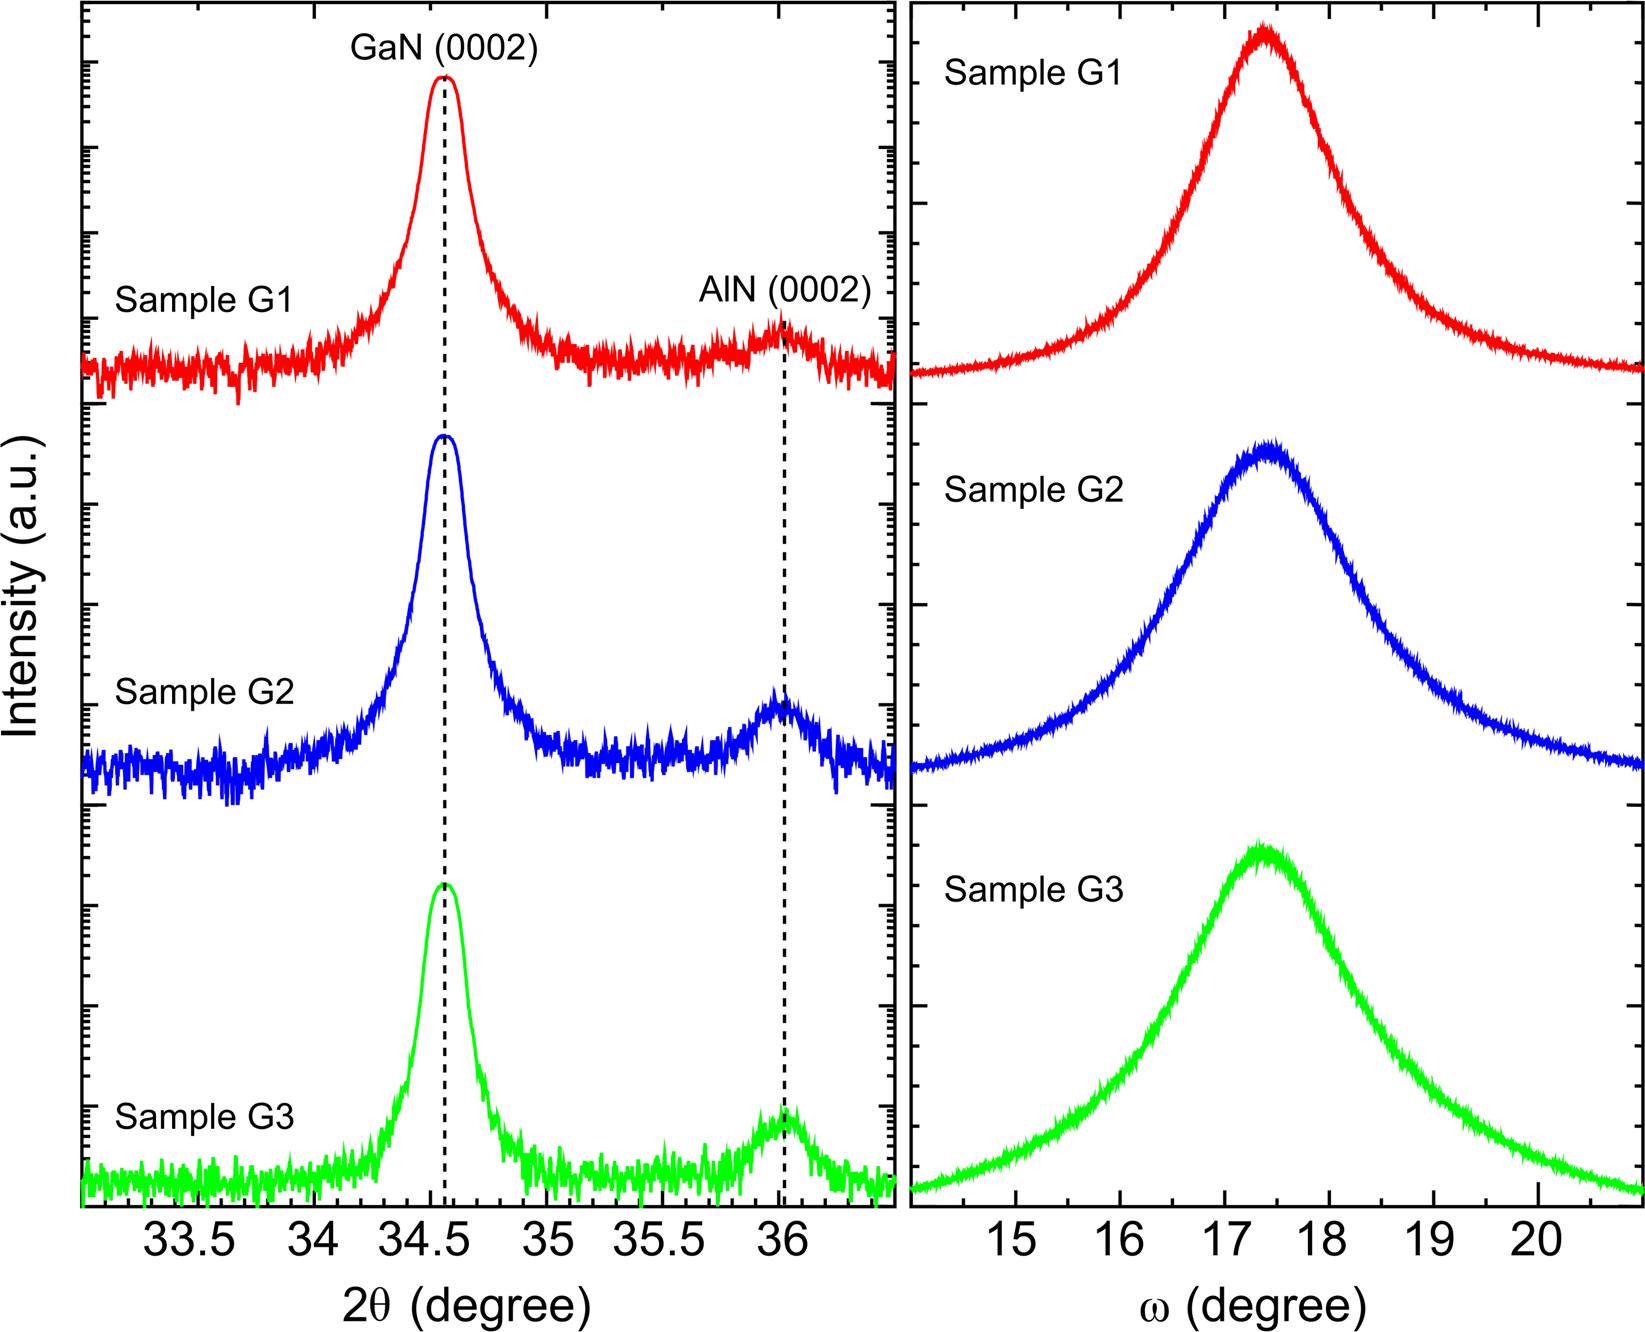
\includegraphics[width=\textwidth]{figures/paper-iv/fig-6.png}
    \caption[HRXRD measurements of the nanocolumns]{HRXRD measurements of the nanocolumns. (\textbf{a}) 2\straighttheta-\textomega \ scanning curve and (\textbf{b}) \textomega \ scanning curve of samples G1, G2 and G3 (adapted with permission from ref. \citenum{liudimulyo2020853} \copyright \ Liudi Mulyo \textit{et al}, 2020.}
    \label{fig:figures/paper-iv/fig-6}
\end{figure}

\section{Section 1 in chapter 6}
\lipsum[2-4]

\subsection{Subsection 6.1 of section 1 in chapter 6}
\lipsum[5-7]

\subsection{Subsection 6.2 of section 1 in chapter 6}
\lipsum[8-11]

\clearpage\phantomsection % to fix wrong hyperref to this section
\section[Long section title displayed in the table of content]{Short section title in the chapter}
\sectionmark{Even shorter title on the header}
\lipsum[11-18]
See \ref{tab:ch6}

\begin{table}[H]
\centering
\caption[Al-content of each axial nanocolumn segment for the vertical GaN/AlGaN nanocolumn ensemble obtained from fitting the simulation model to the HRXRD 2\straighttheta-\textomega \ scan data]{Al-content of each axial nanocolumn segment for the vertical GaN/AlGaN nanocolumn ensemble (top to bottom) obtained from fitting the simulation model to the HRXRD 2\straighttheta-\textomega \ scan data}
\label{tab:ch6}
{\fontsize{7}{6}\selectfont
{\renewcommand{\arraystretch}{2}
\begin{tabular}{cccc}
\textbf{Segment} & \textbf{Thickness (nm)} & \textbf{Al bottom (\%)} & \textbf{Al top (\%)} \\
\midrule
\begin{tabular}[c]{@{}c@{}}\textit{p-}GaN\end{tabular} & 1 & 2 & 3 \\
\rowcolor{Gray}\begin{tabular}[c]{@{}c@{}}\textit{p-}AlGaN (linear grading)\end{tabular} & 4 & 5 & 6 \\
\begin{tabular}[c]{@{}c@{}}\textit{i-}GaN quantum disk\end{tabular} & 7 & 8 & 9 \\
\rowcolor{Gray}\begin{tabular}[c]{@{}c@{}}\textit{n-}AlGaN (linear grading)\end{tabular} & 10 & 11 & 12 \\
\begin{tabular}[c]{@{}c@{}}\textit{n-}GaN\end{tabular} & 13 & 14 & 15 \\
\rowcolor{Gray}\begin{tabular}[c]{@{}c@{}}\textit{n-}AlN buffer layer\end{tabular} & 16 & 17 & 18 \\
\end{tabular}
}
}
\end{table}

\subsection{Subsection 6.2 of section 2 in chapter 6}
\label{subsec:labelsubsec6-2}
\lipsum[13-14]
See \hyperref[appendix:C]{Appendix C} for the \ref{fig:figures/paper-iv/fig-7} and \ref{fig:figures/paper-iv/fig-8}.

%=======================================================================
%%% References 

% \clearpage
\phantomsection
\specialsection % put an indent, see preamble
\headerspecialsection

{\hypersetup{urlcolor=ntnu,linkcolor=sophia} % set clickable URL title color to black, not ntnu like in the main document

\bibliographystyle{unsrtnat-mod}  % NATBIB ref style
\bibliography{references}
}